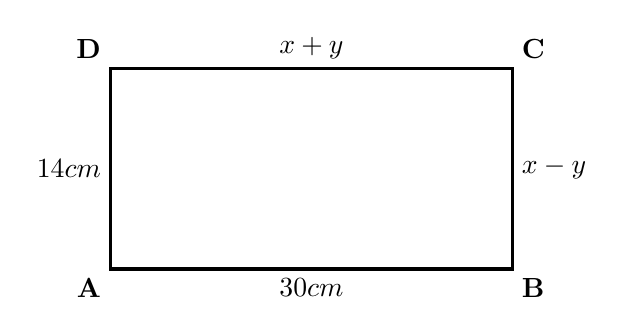
\begin{tikzpicture}[scale=0.85]
    % Draw the rectangle box (width 6, height 3)
    \draw[line width=1.2pt] (0,0) -- (6,0) -- (6,3) -- (0,3) -- cycle;

    % Vertex labels (A, B, C, D)
    \node[below left] at (0,0) {\textbf{A}};
    \node[below right] at (6,0) {\textbf{B}};
    \node[above right] at (6,3) {\textbf{C}};
    \node[above left] at (0,3) {\textbf{D}};

    % Side measurement labels
    \node[below] at (3, 0) {$30\text{ cm}$};
    \node[right] at (6, 1.5) {$x - y$};
    \node[above] at (3, 3) {$x + y$};
    \node[left] at (0, 1.5) {$14\text{ cm}$};
\end{tikzpicture}
